\documentclass{article}
\usepackage{amsmath,amssymb,amsthm,enumitem} % Some standard math packages.
\usepackage{titling} % Enables \setlength{\droptitle}
\usepackage{parskip} % Cleaner paragraph display
\usepackage[margin=1in]{geometry} % Adjusts margins.
\usepackage[utf8]{inputenc} % USe UTF-8 input encoding instead of default ASCII.
\usepackage[]{forest} % Draws trees.
\usepackage{fancyvrb} % Allows Verbatim sections with line numbers and such. Note the capital V.
\usepackage{pgfplots} % For drawing graphs
\usepackage{hyperref} % For hyperlinks
\pgfplotsset{compat=1.6}
\newcommand {\todo}[1] {{\textbf{\color{red}#1}}}

\title{CS 584 Research Project \\ \large Portland State University}
\author{ Dylan Laufenberg }
\date{June 5, 2018}

\begin{document}
\maketitle

\paragraph{Project topic} I will implement a variety of data structures that maintain total orders on their data, e.g. 2-3 trees, treaps, and skip lists; I will choose at least one deterministic structure as a reference and at least one randomized data structure for comparison. I will experimentally evaluate the rates of growth of their run times for insertions, searches, and deletions. Based on these data, I will discuss how the performance I observe compares to the predicted asymptotic performance.

\section{Introduction}
This paper aims to illuminate various facets of the relationship between asymptotic complexity and empirical performance of a range of related data structures. The vehicle for this exploration is a series of benchmarks of data structures that perform similar jobs in very different ways. These include binary search trees, treaps, and skip lists \todo{FINALIZE LIST OF DATA STRUCTURES}. For many tasks, they have the same asymptotic complexity, e.g. average complexity of $O(\log n)$ for search, insert, and delete operations, with worst-case complexity of $O(n)$ for each. This paper examines the performance characteristics of each and investigates how comparable the performance characteristics of these asymptotically equivalent data structures really are.

\section{Testing Methodology}
Gathering reliable data is, of course, of paramount importance to any data-based analysis. Since the analysis in this paper is based on benchmark data, the accuracy of the analysis hinges on the accuracy of the benchmarks themselves. The benchmarks included in this paper utilize the following measures to help ensure their accuracy:

\begin{itemize}
    \item To minimize the impact of timer error, CPU load spikes, and so on, each data point is the average running time of a large number of operations $k$, where $k \geq 100$.
    \item To minimize the impact of such large values of $k$, the overall sample sizes are suitably large, such that $n \geq 100 \cdot k$, where $n$ is the size of a data structure when the $k$ timed operations begin. In other words, the number of operations being timed is no larger than 1\% of the overall data structure at any point.
    \item When necessary for accuracy, multiple passes may be combined by taking the median or mean time of the running times for each value of $n$ being plotted.
    \item Since these benchmarks are highly sensitive to fluctuating operating conditions (e.g. CPU scheduling, RAM availability, and Python interpreter behavior), each benchmark produces multiple graphs. The most representative graph among the set is chosen for inclusion in this paper.
    \item To prevent human error in transcribing graphs or plot data, all graphs are generated programmatically using the same function and included without modification (except to specify each graph's placement and size).
\end{itemize}

\emph{Note that some of the graphs under \todo{TESTING DATA STRUCTURES SECTION NAME} necessarily disobey the above guidelines.}

\section{Project Files}
The Python 3 implementations included with this report are structured as follows:
\begin{itemize}
    \item datastructures/ --- contains the implementations of data structures benchmarked below, one per file.
    \item plots/ --- contains the output \LaTeX \ figures that the benchmark system produces, ready to \\include.
    \item pgfplot.py --- contains the PgfPlot class, which represents one \LaTeX \ figure to be produced. This class receives and stores all parameters that affect the figure, including plots to be produced.
    \item plot.py --- contains the Plot and BenchmarkPlot classes, which represent plots in a PGFPLOT graph. The Plot class may be used to produce arbitrary plots, whereas the BenchmarkPlot class receives benchmark parameters for one function and produces the corresponding plot.
    \item benchmark.py --- sets up and runs the benchmarks used in this document by creating PgfPlot objects and running them.
\end{itemize}

To run custom benchmarks, simply follow the examples in benchmark.py. All classes are thoroughly documented and commented.

\section{Data Structure Selection}
Many implementations exist for each of these data structures, since they are well-known. 

\section{Data Structure Implementations}
All credit for implementations go to the authors of the respective data structure implementations. All data structures used are cited here.

\begin{itemize}
    \item binarysearchtree.py --- Dylan Laufenberg (written as a naive reference for these benchmarks)
    \item toastdriven\_pyskip.py --- Credit: Daniel Lindsley. Modified from \url{https://github.com/toastdriven/pyskip}.
    \item stromberg\_treap.py --- Credit: Dan Stromberg. Modified from \url{https://pypi.org/project/treap/}.
    \item jenks\_treap.py --- Credit: Grant Jenks. Modified from \url{http://www.grantjenks.com/wiki/random/python_treap_implementation}. Converted from Python 2 to Python 3.
    \item pyskiplist/ --- Credit: Geert Jansen. Modified from \url{https://pypi.org/project/pyskiplist/}.
\end{itemize}

The above data structures have been modified as needed to standardize their interfaces for insert, search, and delete operations.

\todo{Charts here comparing different implementations of various data structures}

\todo{Section: Asymptotic Expectations - talk about expected/average performance.}
\newpage
\section{Testing TikZ Pictures}

\begin{figure}[h]
    \centering
    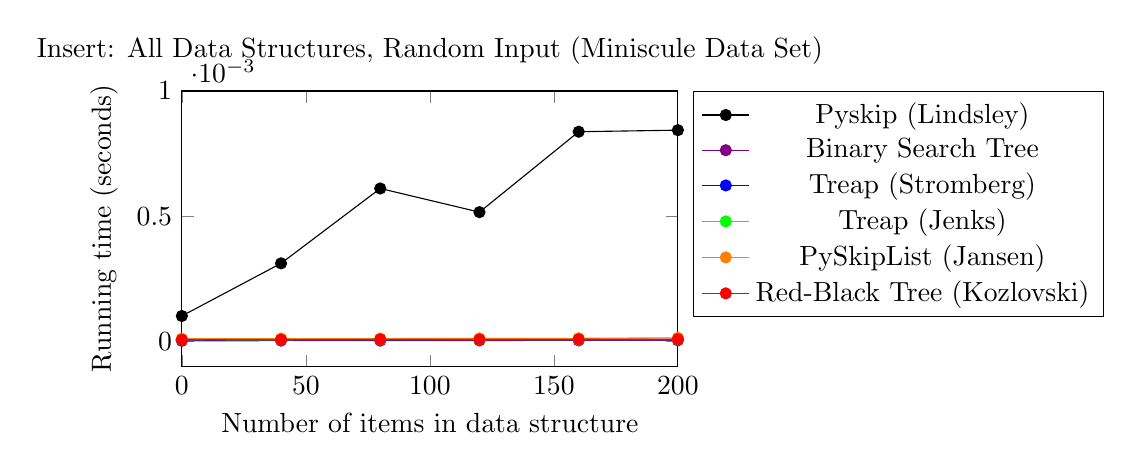
\begin{tikzpicture}
        \begin{axis}[
            title={Insert: All Data Structures, Random Input (Miniscule Data Set)},
            xmin=0, xmax=200,
            ymin=-0.0001, ymax=0.0010,
            xlabel={Number of items in data structure},
            ylabel={Running time (seconds)},
            width=0.65\textwidth,
            height=2in,
            legend pos=outer north east,
        ]
		% Pyskip
		\addplot[
		    color=black, 
		    mark=*,
	    ]
		coordinates {
			(0, 0.00010143585341796358)
			(40, 0.000311535768335931)
			(80, 0.0006105426426629923)
			(120, 0.0005160940570576679)
			(160, 0.0008371770835686271)
			(200, 0.0008434114130393855)
		};
        % BST
		\addplot[
		    color=violet,
		    mark=*,
	    ]
		coordinates {
			(0, 2.1082273572617137e-06)
			(40, 2.8912832328160653e-06)
			(80, 2.9816358338415635e-06)
			(120, 3.6743391083704157e-06)
			(160, 3.7646917093959164e-06)
			(200, 3.794809243071076e-06)
		};
		% Stromberg treap
		\addplot[
		    color=blue,
		    mark=*,
	    ]
        coordinates {
			(0, 5.1500982584523625e-06)
			(40, 6.6559749422101525e-06)
			(80, 6.3849171391350264e-06)
			(120, 6.987267812638698e-06)
			(160, 7.318560683064468e-06)
			(200, 7.288443149391921e-06)
		};
		% Jenks treap
		\addplot[
		    color=green,
		    mark=*,
	    ]
		coordinates {
			(0, 6.776445076911442e-06)
			(40, 6.625857408537605e-06)
			(80, 7.318560683064468e-06)
			(120, 6.9270327452880535e-06)
			(160, 6.776445076911442e-06)
			(200, 7.318560683064468e-06)
		};
		% PySkipList
		\addplot[
		    color=orange,
		    mark=*,
	    ]
         coordinates {
			(0, 1.0511019252634756e-05)
			(40, 1.1294075128187587e-05)
			(80, 1.108325239246033e-05)
			(120, 1.1986778402717224e-05)
			(160, 1.2287953739470447e-05)
			(200, 1.424559342835252e-05)
		};
		% Red-black tree
		\addplot[
		    color=red, 
		    mark=*,
	    ]
         coordinates {
			(0, 6.8366801442620865e-06)
			(40, 6.776445076911442e-06)
			(80, 8.101616558620073e-06)
			(120, 7.348678216742566e-06)
			(160, 8.342556828022651e-06)
			(200, 8.463026962721166e-06)
		};
        \legend{Pyskip (Lindsley), Binary Search Tree, Treap (Stromberg), Treap (Jenks), PySkipList (Jansen), Red-Black Tree (Kozlovski)}
        \end{axis}
    \end{tikzpicture}
    \caption{Average of 10 operations, benchmarked every 40, starting at 0.}
\end{figure}
\begin{figure}[h]
    \centering
    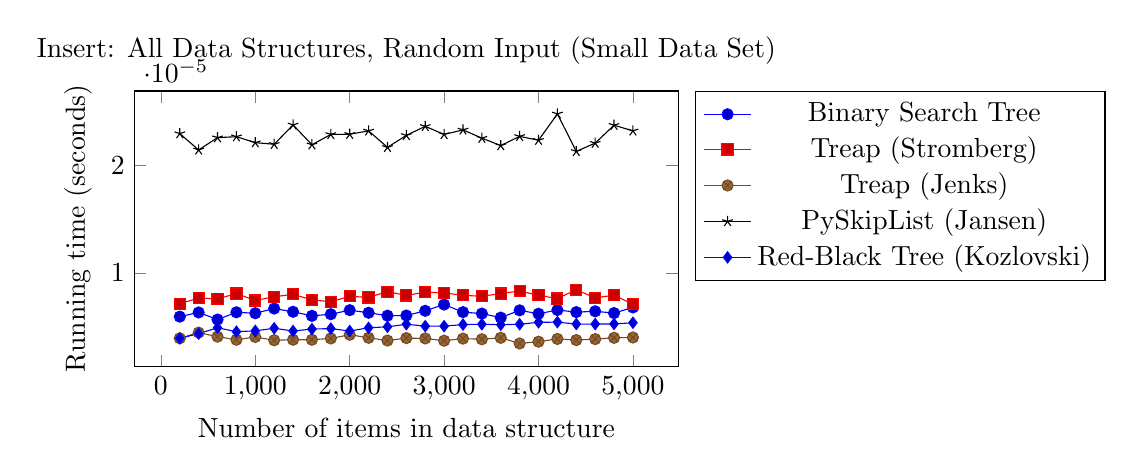
\begin{tikzpicture}
        \begin{axis}[
            xlabel={Number of items in data structure},
            ylabel={Running time (seconds)},
            title={Insert: All Data Structures, Random Input (Small Data Set)},
            width=0.7\textwidth,
            height=2in,
            legend pos=outer north east
        ]
		\addplot coordinates {
			(200, 5.933154134041274e-06)
			(400, 6.324682071845444e-06)
			(600, 5.662096330993905e-06)
			(800, 6.3397408387011465e-06)
			(1000, 6.249388237655751e-06)
			(1200, 6.686092475849392e-06)
			(1400, 6.384917139090618e-06)
			(1600, 6.00844796814215e-06)
			(1800, 6.159035636521537e-06)
			(2000, 6.535504807558823e-06)
			(2200, 6.29456453813404e-06)
			(2400, 6.023506734997852e-06)
			(2600, 6.0385655018535545e-06)
			(2800, 6.475269740136014e-06)
			(3000, 7.062561646886678e-06)
			(3200, 6.354799605468031e-06)
			(3400, 6.219270703944346e-06)
			(3600, 5.842801532995878e-06)
			(3800, 6.520446040703121e-06)
			(4000, 6.204211937088644e-06)
			(4200, 6.550563574414525e-06)
			(4400, 6.354799605468031e-06)
			(4600, 6.430093439568907e-06)
			(4800, 6.264447004422635e-06)
			(5000, 6.7915038437504904e-06)
		};
		\addplot coordinates {
			(200, 7.137855480987554e-06)
			(400, 7.664912320315409e-06)
			(600, 7.5896184861257154e-06)
			(800, 8.086557791830984e-06)
			(1000, 7.439030817746328e-06)
			(1200, 7.785382454983391e-06)
			(1400, 8.01126395764129e-06)
			(1600, 7.499265885169137e-06)
			(1800, 7.318560683078346e-06)
			(2000, 7.830558755550498e-06)
			(2200, 7.7251473876494e-06)
			(2400, 8.267262993832958e-06)
			(2600, 7.905852589740191e-06)
			(2800, 8.222086693265851e-06)
			(3000, 8.146792859164976e-06)
			(3200, 7.920911356507076e-06)
			(3400, 7.830558755550498e-06)
			(3600, 8.086557791742166e-06)
			(3800, 8.327498061166948e-06)
			(4000, 7.920911356595894e-06)
			(4200, 7.61973601983712e-06)
			(4400, 8.43290942897923e-06)
			(4600, 7.695029853937996e-06)
			(4800, 7.920911356595894e-06)
			(5000, 7.092679180509265e-06)
		};
		\addplot coordinates {
			(200, 3.915279377775249e-06)
			(400, 4.4423362171031044e-06)
			(600, 4.0658670461546365e-06)
			(800, 3.7797504762515643e-06)
			(1000, 4.035749512443232e-06)
			(1200, 3.7345741756844575e-06)
			(1400, 3.7797504761627465e-06)
			(1600, 3.7797504762515643e-06)
			(1800, 3.900220611008365e-06)
			(2000, 4.246572248156611e-06)
			(2200, 3.960455678342356e-06)
			(2400, 3.7044566420618706e-06)
			(2600, 3.930338144630951e-06)
			(2800, 3.900220610919547e-06)
			(3000, 3.6893978752061685e-06)
			(3200, 3.885161844152662e-06)
			(3400, 3.824926776729854e-06)
			(3600, 3.960455678342356e-06)
			(3800, 3.433398838925683e-06)
			(4000, 3.5990452741607727e-06)
			(4200, 3.855044310441258e-06)
			(4400, 3.7496329425401596e-06)
			(4600, 3.839985543585556e-06)
			(4800, 3.960455678253538e-06)
			(5000, 3.990573211964943e-06)
		};
		\addplot coordinates {
			(200, 2.2994736960946228e-05)
			(400, 2.147380151038547e-05)
			(600, 2.261826778999776e-05)
			(800, 2.2708620391043154e-05)
			(1000, 2.2151446018092714e-05)
			(1200, 2.2000858349713327e-05)
			(1400, 2.3807910370177156e-05)
			(1600, 2.195568204914622e-05)
			(1800, 2.2919443126845353e-05)
			(2000, 2.2934501893612236e-05)
			(2200, 2.3250735997226712e-05)
			(2400, 2.1714741779810254e-05)
			(2600, 2.2829090525799955e-05)
			(2800, 2.367238146865347e-05)
			(3000, 2.2919443126845353e-05)
			(3200, 2.334108859827211e-05)
			(3400, 2.257309148951947e-05)
			(3600, 2.1880388215045343e-05)
			(3800, 2.273873792475456e-05)
			(4000, 2.2377327520661795e-05)
			(4200, 2.483190651512146e-05)
			(4400, 2.1338272608861786e-05)
			(4600, 2.2106269717614425e-05)
			(4800, 2.3777792836554566e-05)
			(5000, 2.3250735997226712e-05)
		};
		\addplot coordinates {
			(200, 3.915279377775249e-06)
			(400, 4.351983616057708e-06)
			(600, 4.894099222241266e-06)
			(800, 4.5326888180596825e-06)
			(1000, 4.607982652338194e-06)
			(1200, 4.848922921762977e-06)
			(1400, 4.592923885482492e-06)
			(1600, 4.773629087484465e-06)
			(1800, 4.8188053880515724e-06)
			(2000, 4.592923885393674e-06)
			(2200, 4.894099222241266e-06)
			(2400, 4.984451823286662e-06)
			(2600, 5.225392092622627e-06)
			(2800, 5.044686890620653e-06)
			(3000, 5.044686890620653e-06)
			(3200, 5.1952745590000404e-06)
			(3400, 5.225392092622627e-06)
			(3600, 5.180215792144338e-06)
			(3800, 5.225392092711445e-06)
			(4000, 5.406097294713419e-06)
			(4200, 5.421156061480304e-06)
			(4400, 5.2404508594783294e-06)
			(4600, 5.2404508594783294e-06)
			(4800, 5.2555096263340316e-06)
			(5000, 5.360920994146312e-06)
		};
        \legend{Binary Search Tree, Treap (Stromberg), Treap (Jenks), PySkipList (Jansen), Red-Black Tree (Kozlovski)}
        \end{axis}
    \end{tikzpicture}
    \caption{Average of 20 operations, benchmarked every 200, starting at 200.}
\end{figure}

\begin{figure}[h]
    \centering
    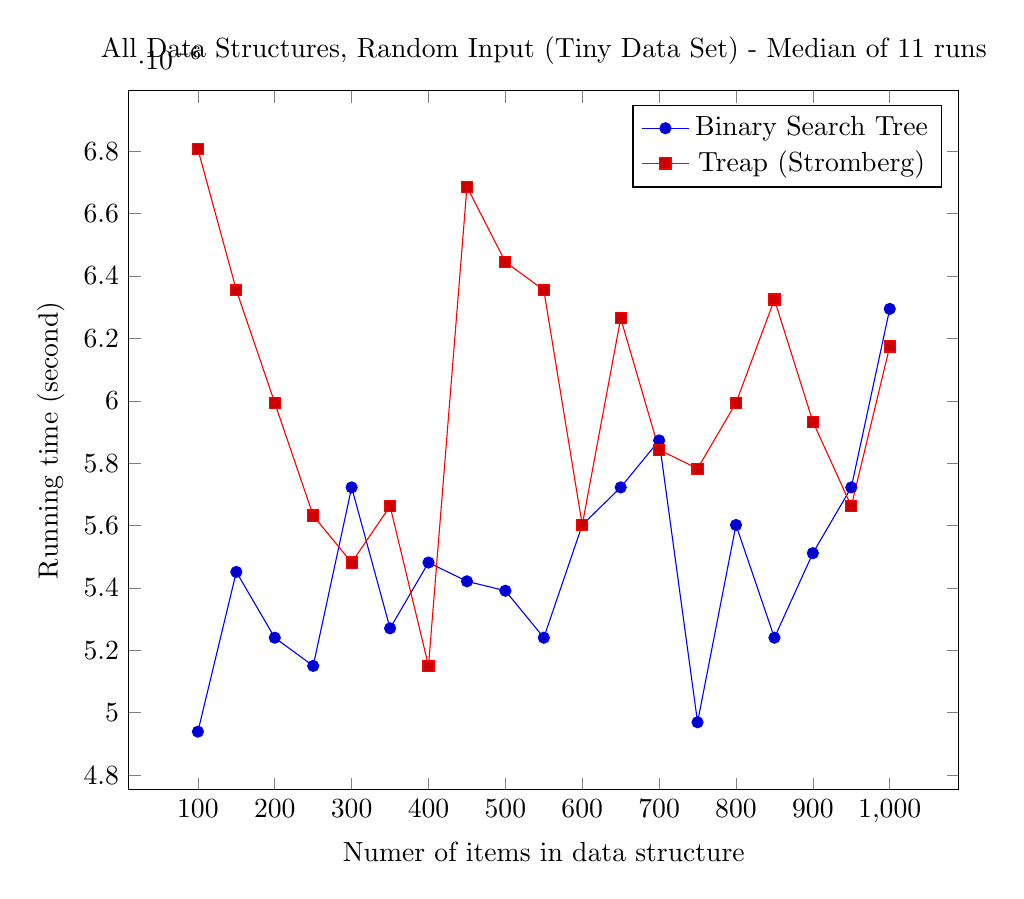
\begin{tikzpicture}
        \begin{axis}[
            xlabel={Numer of items in data structure},
            ylabel={Running time (second)},
            title={All Data Structures, Random Input (Tiny Data Set) - Median of 11 runs},
            width=\textwidth
        ]
		\addplot coordinates {
			(100, 4.939275522719555e-06)
			(150, 5.451273595191708e-06)
			(200, 5.2404508594783294e-06)
			(250, 5.150098258432933e-06)
			(300, 5.722331398283487e-06)
			(350, 5.2705683931453254e-06)
			(400, 5.481391128903112e-06)
			(450, 5.421156061524712e-06)
			(500, 5.391038527857717e-06)
			(550, 5.2404508594783294e-06)
			(600, 5.601861263571095e-06)
			(650, 5.722331398283487e-06)
			(700, 5.872919066618465e-06)
			(750, 4.969393056386551e-06)
			(800, 5.601861263571095e-06)
			(850, 5.2404508594783294e-06)
			(900, 5.511508662570108e-06)
			(950, 5.722331398283487e-06)
			(1000, 6.294564538089631e-06)
		};
		\addplot coordinates {
			(100, 6.8065626106061926e-06)
			(150, 6.354799605468031e-06)
			(200, 5.993389201330856e-06)
			(250, 5.6319787972824996e-06)
			(300, 5.481391128858704e-06)
			(350, 5.6620963309494956e-06)
			(400, 5.150098258432933e-06)
			(450, 6.686092475893801e-06)
			(500, 6.4451522064690184e-06)
			(550, 6.354799605468031e-06)
			(600, 5.601861263615504e-06)
			(650, 6.264447004467044e-06)
			(700, 5.842801532995878e-06)
			(750, 5.782566465617478e-06)
			(800, 5.993389201330856e-06)
			(850, 6.324682071801035e-06)
			(900, 5.933154133996865e-06)
			(950, 5.6620963309050865e-06)
			(1000, 6.174094403421648e-06)
		};
        \legend{Binary Search Tree, Treap (Stromberg)}
        \end{axis}
    \end{tikzpicture}
    \caption{Average of 10 operations, benchmarked every 50, starting at 100. Median of 11 runs.}
\end{figure}
\begin{figure}[h]
    \centering
    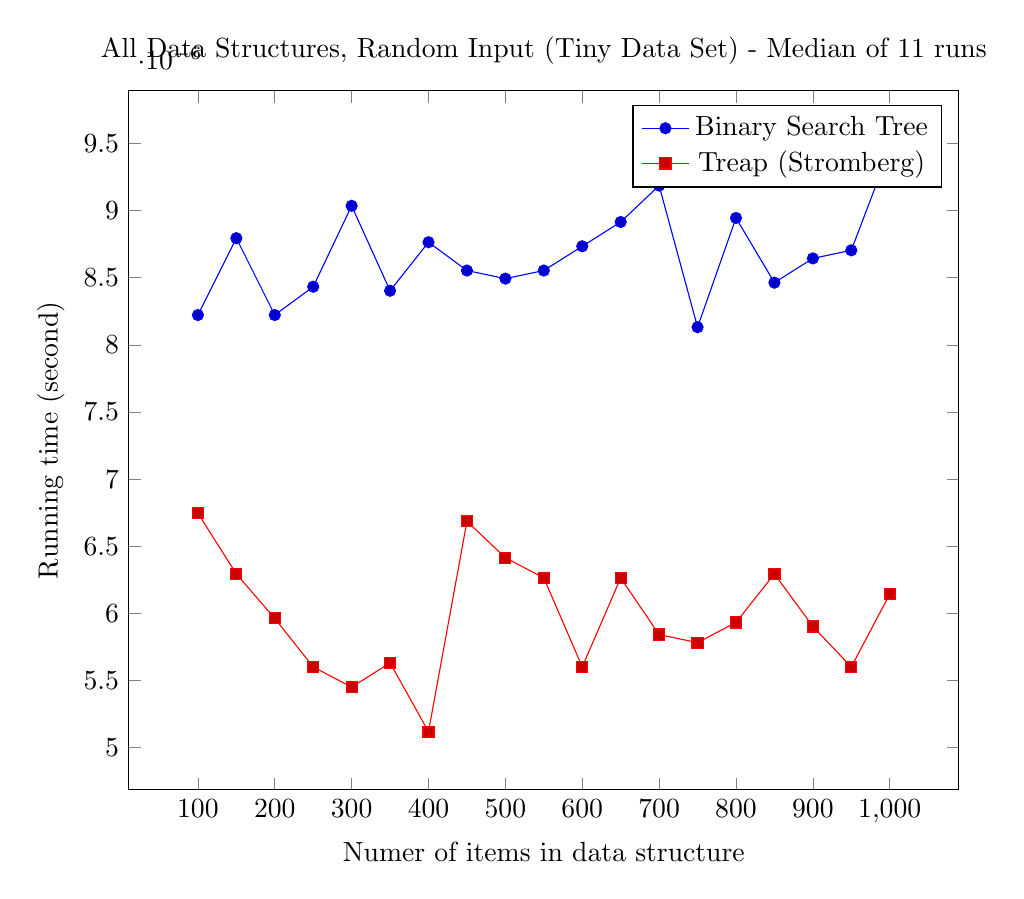
\begin{tikzpicture}
        \begin{axis}[
            xlabel={Numer of items in data structure},
            ylabel={Running time (second)},
            title={All Data Structures, Random Input (Tiny Data Set) - Median of 11 runs},
            width=\textwidth
        ]
		\addplot coordinates {
			(100, 8.22208669331026e-06)
			(150, 8.794319833160813e-06)
			(200, 8.222086693354669e-06)
			(250, 8.432909429023638e-06)
			(300, 9.035260102541187e-06)
			(350, 8.402791895401052e-06)
			(400, 8.764202299449408e-06)
			(450, 8.55337956373603e-06)
			(500, 8.493144496402038e-06)
			(550, 8.553379563780438e-06)
			(600, 8.734084765782412e-06)
			(650, 8.914789967873205e-06)
			(700, 9.185847770920574e-06)
			(750, 8.131734092309273e-06)
			(800, 8.944907501495791e-06)
			(850, 8.463026962690634e-06)
			(900, 8.643732164781426e-06)
			(950, 8.703967232115416e-06)
			(1000, 9.456905573967944e-06)
		};
		\addplot coordinates {
			(100, 6.746327543272201e-06)
			(150, 6.29456453813404e-06)
			(200, 5.9632716677082694e-06)
			(250, 5.601861263571095e-06)
			(300, 5.451273595191708e-06)
			(350, 5.6319787972824996e-06)
			(400, 5.119980724765938e-06)
			(450, 6.686092475893801e-06)
			(500, 6.4150346728020224e-06)
			(550, 6.264447004422635e-06)
			(600, 5.601861263615504e-06)
			(650, 6.264447004422635e-06)
			(700, 5.842801532995878e-06)
			(750, 5.782566465617478e-06)
			(800, 5.933154133996865e-06)
			(850, 6.294564538089631e-06)
			(900, 5.903036600329869e-06)
			(950, 5.601861263571095e-06)
			(1000, 6.143976869710244e-06)
		};
        \legend{Binary Search Tree, Treap (Stromberg)}
        \end{axis}
    \end{tikzpicture}
    \caption{Average of 10 operations, benchmarked every 50, starting at 100. Median of 11 runs.}
\end{figure}
\begin{figure}[h]
    \centering
    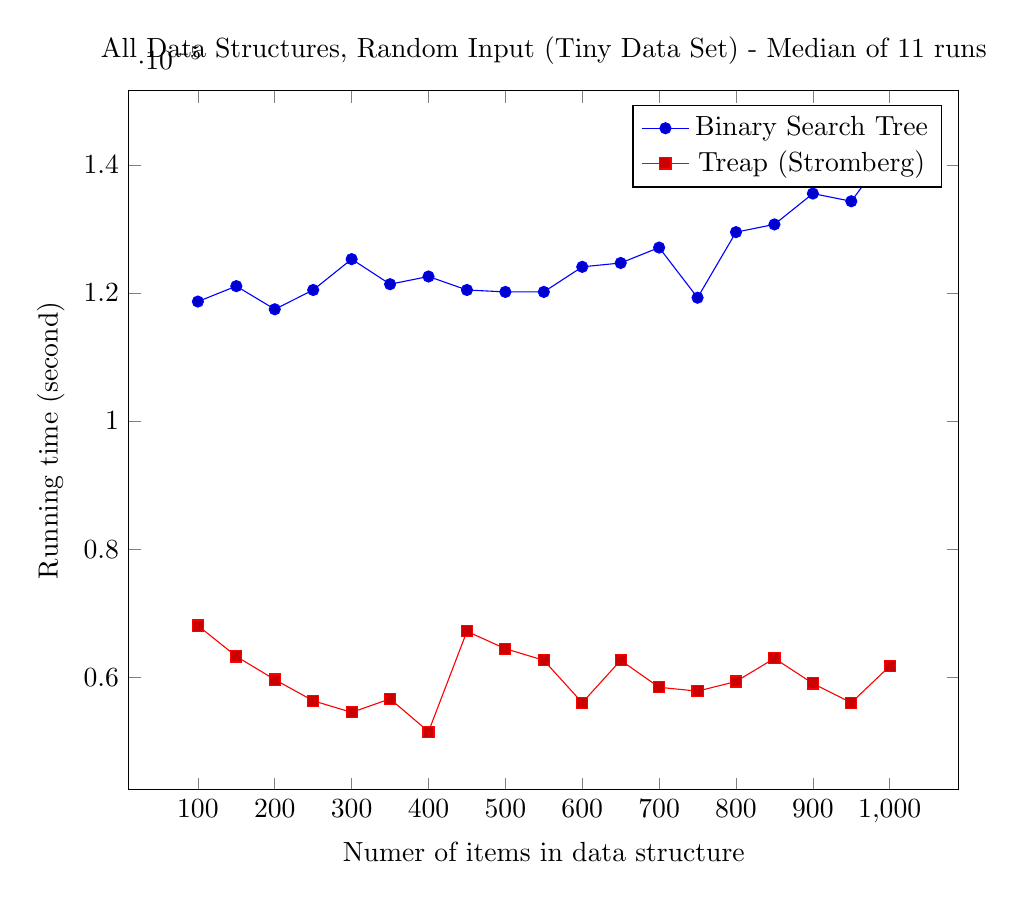
\begin{tikzpicture}
        \begin{axis}[
            xlabel={Numer of items in data structure},
            ylabel={Running time (second)},
            title={All Data Structures, Random Input (Tiny Data Set) - Median of 11 runs},
            width=\textwidth
        ]
		\addplot coordinates {
			(100, 1.1866308268038139e-05)
			(150, 1.2107248537418513e-05)
			(200, 1.1745838133281338e-05)
			(250, 1.2047013470084523e-05)
			(300, 1.252889400884527e-05)
			(350, 1.2137366071085509e-05)
			(400, 1.2257836205797901e-05)
			(450, 1.2047013470040113e-05)
			(500, 1.2016895936417527e-05)
			(550, 1.2016895936373117e-05)
			(600, 1.2408423874177288e-05)
			(650, 1.246865894151128e-05)
			(700, 1.2709599210936063e-05)
			(750, 1.192654333537213e-05)
			(800, 1.2950539480316437e-05)
			(850, 1.3071009615028828e-05)
			(900, 1.3552890153833985e-05)
			(950, 1.3432420019121594e-05)
			(1000, 1.424559342835252e-05)
		};
		\addplot coordinates {
			(100, 6.8065626106061926e-06)
			(150, 6.324682071845444e-06)
			(200, 5.963271667663861e-06)
			(250, 5.6319787972824996e-06)
			(300, 5.451273595191708e-06)
			(350, 5.662096330993905e-06)
			(400, 5.150098258432933e-06)
			(450, 6.716210009560797e-06)
			(500, 6.445152206424609e-06)
			(550, 6.264447004511453e-06)
			(600, 5.601861263571095e-06)
			(650, 6.264447004422635e-06)
			(700, 5.842801532995878e-06)
			(750, 5.782566465661887e-06)
			(800, 5.933154134041274e-06)
			(850, 6.29456453813404e-06)
			(900, 5.903036600329869e-06)
			(950, 5.601861263571095e-06)
			(1000, 6.174094403466057e-06)
		};
        \legend{Binary Search Tree, Treap (Stromberg)}
        \end{axis}
    \end{tikzpicture}
    \caption{Average of 10 operations, benchmarked every 50, starting at 100. Median of 11 runs.}
\end{figure}
\begin{figure}[h]
    \centering
    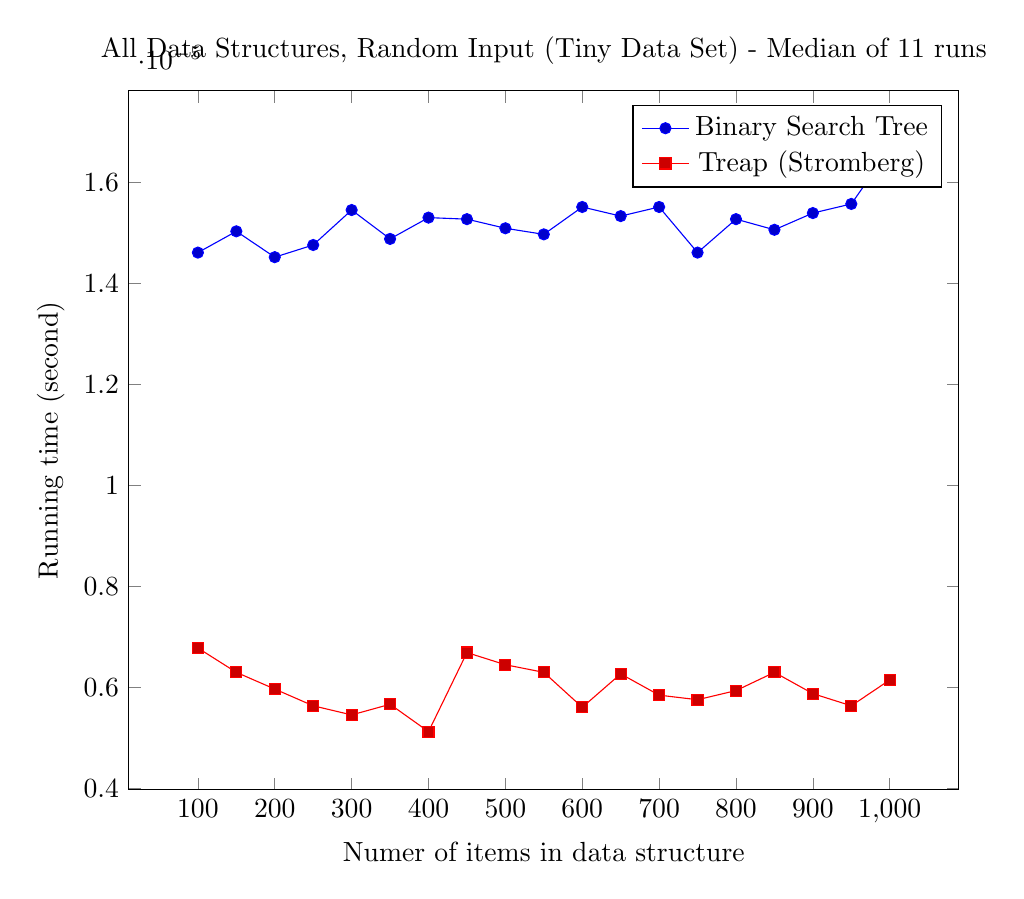
\begin{tikzpicture}
        \begin{axis}[
            xlabel={Numer of items in data structure},
            ylabel={Running time (second)},
            title={All Data Structures, Random Input (Tiny Data Set) - Median of 11 runs},
            width=\textwidth
        ]
		\addplot coordinates {
			(100, 1.4607003832445287e-05)
			(150, 1.5028649303872044e-05)
			(200, 1.4516651231399891e-05)
			(250, 1.4757591500824674e-05)
			(300, 1.5450294775387618e-05)
			(350, 1.4878061635492656e-05)
			(400, 1.5299707106919415e-05)
			(450, 1.5269589573296825e-05)
			(500, 1.5088884371294853e-05)
			(550, 1.4968414236538052e-05)
			(600, 1.551052984272161e-05)
			(650, 1.5329824640630817e-05)
			(700, 1.551052984272161e-05)
			(750, 1.4607003832445287e-05)
			(800, 1.5269589573296825e-05)
			(850, 1.5058766837583449e-05)
			(900, 1.539005970796481e-05)
			(950, 1.5570764910055602e-05)
			(1000, 1.6654996122333897e-05)
		};
		\addplot coordinates {
			(100, 6.776445076894788e-06)
			(150, 6.29456453813404e-06)
			(200, 5.963271667663861e-06)
			(250, 5.631978797193682e-06)
			(300, 5.451273595191708e-06)
			(350, 5.662096330993905e-06)
			(400, 5.119980724810347e-06)
			(450, 6.68609247593821e-06)
			(500, 6.445152206513427e-06)
			(550, 6.29456453813404e-06)
			(600, 5.601861263571095e-06)
			(650, 6.264447004422635e-06)
			(700, 5.842801532995878e-06)
			(750, 5.752448931950483e-06)
			(800, 5.933154134041274e-06)
			(850, 6.29456453813404e-06)
			(900, 5.872919066707283e-06)
			(950, 5.6319787972824996e-06)
			(1000, 6.143976869754653e-06)
		};
        \legend{Binary Search Tree, Treap (Stromberg)}
        \end{axis}
    \end{tikzpicture}
    \caption{Average of 10 operations, benchmarked every 50, starting at 100. Median of 11 runs.}
\end{figure}
\begin{figure}[h]
    \centering
    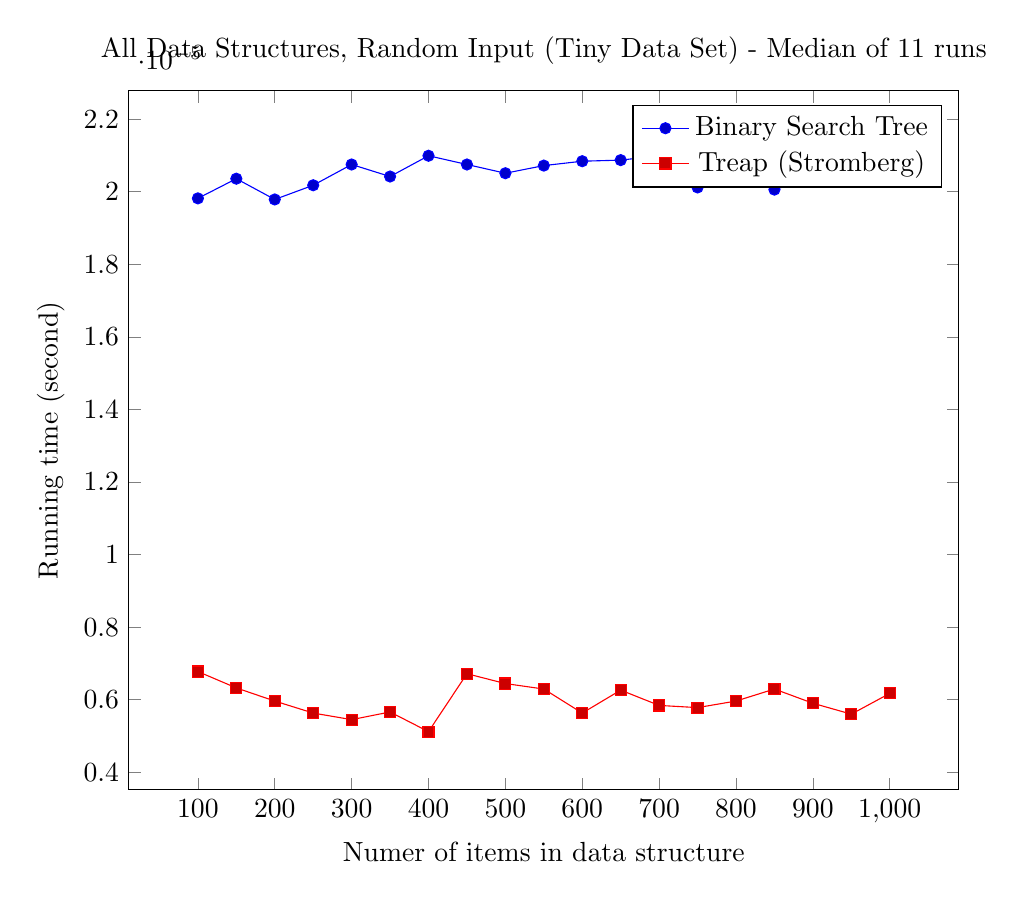
\begin{tikzpicture}
        \begin{axis}[
            xlabel={Numer of items in data structure},
            ylabel={Running time (second)},
            title={All Data Structures, Random Input (Tiny Data Set) - Median of 11 runs},
            width=\textwidth
        ]
		\addplot coordinates {
			(100, 1.981733715830103e-05)
			(150, 2.035945276439577e-05)
			(200, 1.9787219624589625e-05)
			(250, 2.0178747562304976e-05)
			(300, 2.075098070219994e-05)
			(350, 2.0419687831818577e-05)
			(400, 2.0991920971624724e-05)
			(450, 2.075098070219994e-05)
			(500, 2.0510040432775155e-05)
			(550, 2.0720863168577353e-05)
			(600, 2.0841333303156517e-05)
			(650, 2.0871450836867923e-05)
			(700, 2.0991920971535904e-05)
			(750, 2.0118512494970987e-05)
			(800, 2.0660628101154545e-05)
			(850, 2.0058277427636995e-05)
			(900, 2.0389570298018354e-05)
			(950, 2.0389570298107174e-05)
			(1000, 2.1172626173626696e-05)
		};
		\addplot coordinates {
			(100, 6.776445076894788e-06)
			(150, 6.324682071756626e-06)
			(200, 5.963271667663861e-06)
			(250, 5.631978797193682e-06)
			(300, 5.451273595191708e-06)
			(350, 5.662096330993905e-06)
			(400, 5.119980724810347e-06)
			(450, 6.716210009560797e-06)
			(500, 6.445152206424609e-06)
			(550, 6.29456453813404e-06)
			(600, 5.631978797193682e-06)
			(650, 6.264447004422635e-06)
			(700, 5.842801532995878e-06)
			(750, 5.782566465661887e-06)
			(800, 5.963271667663861e-06)
			(850, 6.29456453813404e-06)
			(900, 5.903036600329869e-06)
			(950, 5.601861263571095e-06)
			(1000, 6.17409440337724e-06)
		};
        \legend{Binary Search Tree, Treap (Stromberg)}
        \end{axis}
    \end{tikzpicture}
    \caption{Average of 10 operations, benchmarked every 50, starting at 100. Median of 11 runs.}
\end{figure}

%\comparegraphs{randomAllTiny}
%\comparegraphs{randomAllTinyRepeat}
%\comparegraphs{randomAllSmall}

\end{document}
